\setlength{\parskip}{\baselineskip} 
\section{Conclusion}

\frame{
\frametitle{Comparison: Head to head}
\vspace{1em}
\begin{columns}[t]
\column{.5\textwidth}
\centering{\color{matbluedark}\textbf{PCP-LOD}}
\vspace{1ex}
\begin{itemize}
    \item[$\checkmark$] Not influenced by outliers
    \item[$\checkmark$] Captures extreme events
    \item[$\checkmark$] Modified for values $<$ LOD
    \item[$\checkmark$] Cross-validation chooses number of patterns
    \vspace{1em}
    \item[\xmark] Does not estimate loadings \& scores directly
\end{itemize}
\column{.5\textwidth}
\centering{\color{matbluedark}\textbf{\bnmf}}
\vspace{1ex}
\begin{itemize}
    \item[$\checkmark$] Estimates loadings \& scores directly
    \item[$\checkmark$] Quantifies uncertainty
    \item[$\checkmark$] Determines number of patterns
    \vspace{1em}
    \item[\xmark] No modifications for values $<$ LOD or outliers
    
\end{itemize}
\end{columns}
}

\frame{
\frametitle{Challenges \& next steps}
\vspace{2em}
\begin{columns}
\column{.5\textwidth}
\centering{\color{matbluedark}\textbf{PCP-LOD}}
\vspace{0.5ex}
\begin{itemize}
    \item Estimate scores \& loadings
    \item What to do with sparse matrix?
\end{itemize}
\vspace{1ex}
\centering{\color{matbluedark}\textbf{\bnmf}}
\vspace{0.5ex}
\begin{itemize}
    \item MCMC $\mathbf{\rightarrow}$ better 95\% CI coverage
    \item Fully supervised model
\end{itemize}
\vspace{1ex}
\centering{\color{matbluedark}\textbf{--- --- --- --- --- --- --- --- --- --- --- --- \\
\vspace{1ex}
R packages for both!}}
\column{.5\textwidth}
\onslide\centering{{
\includegraphics[scale=.4]{figures/rcartoon.png}}}
\end{columns}
}

\frame{
\frametitle{Conclusion: What did she say?}
\begin{columns}
\column{.5\textwidth}
\begin{changemargin}{-1em}{0em}
\vspace{1em}
\begin{itemize}
    \item No statistical method answers all research questions
    \item Multi-pollutant exposures require novel methods
    \item Pattern recognition adapted for environmental health 
    \begin{itemize}
        \item Removed the researcher from pattern number selection
        \item Emphasized interpretability of results
        \item Accounted for uncertainty in identified patterns
    \end{itemize}
\end{itemize}
\end{changemargin}
\column{.5\textwidth}
\onslide\begin{changemargin}{-2em}{0em}
\only<1>{{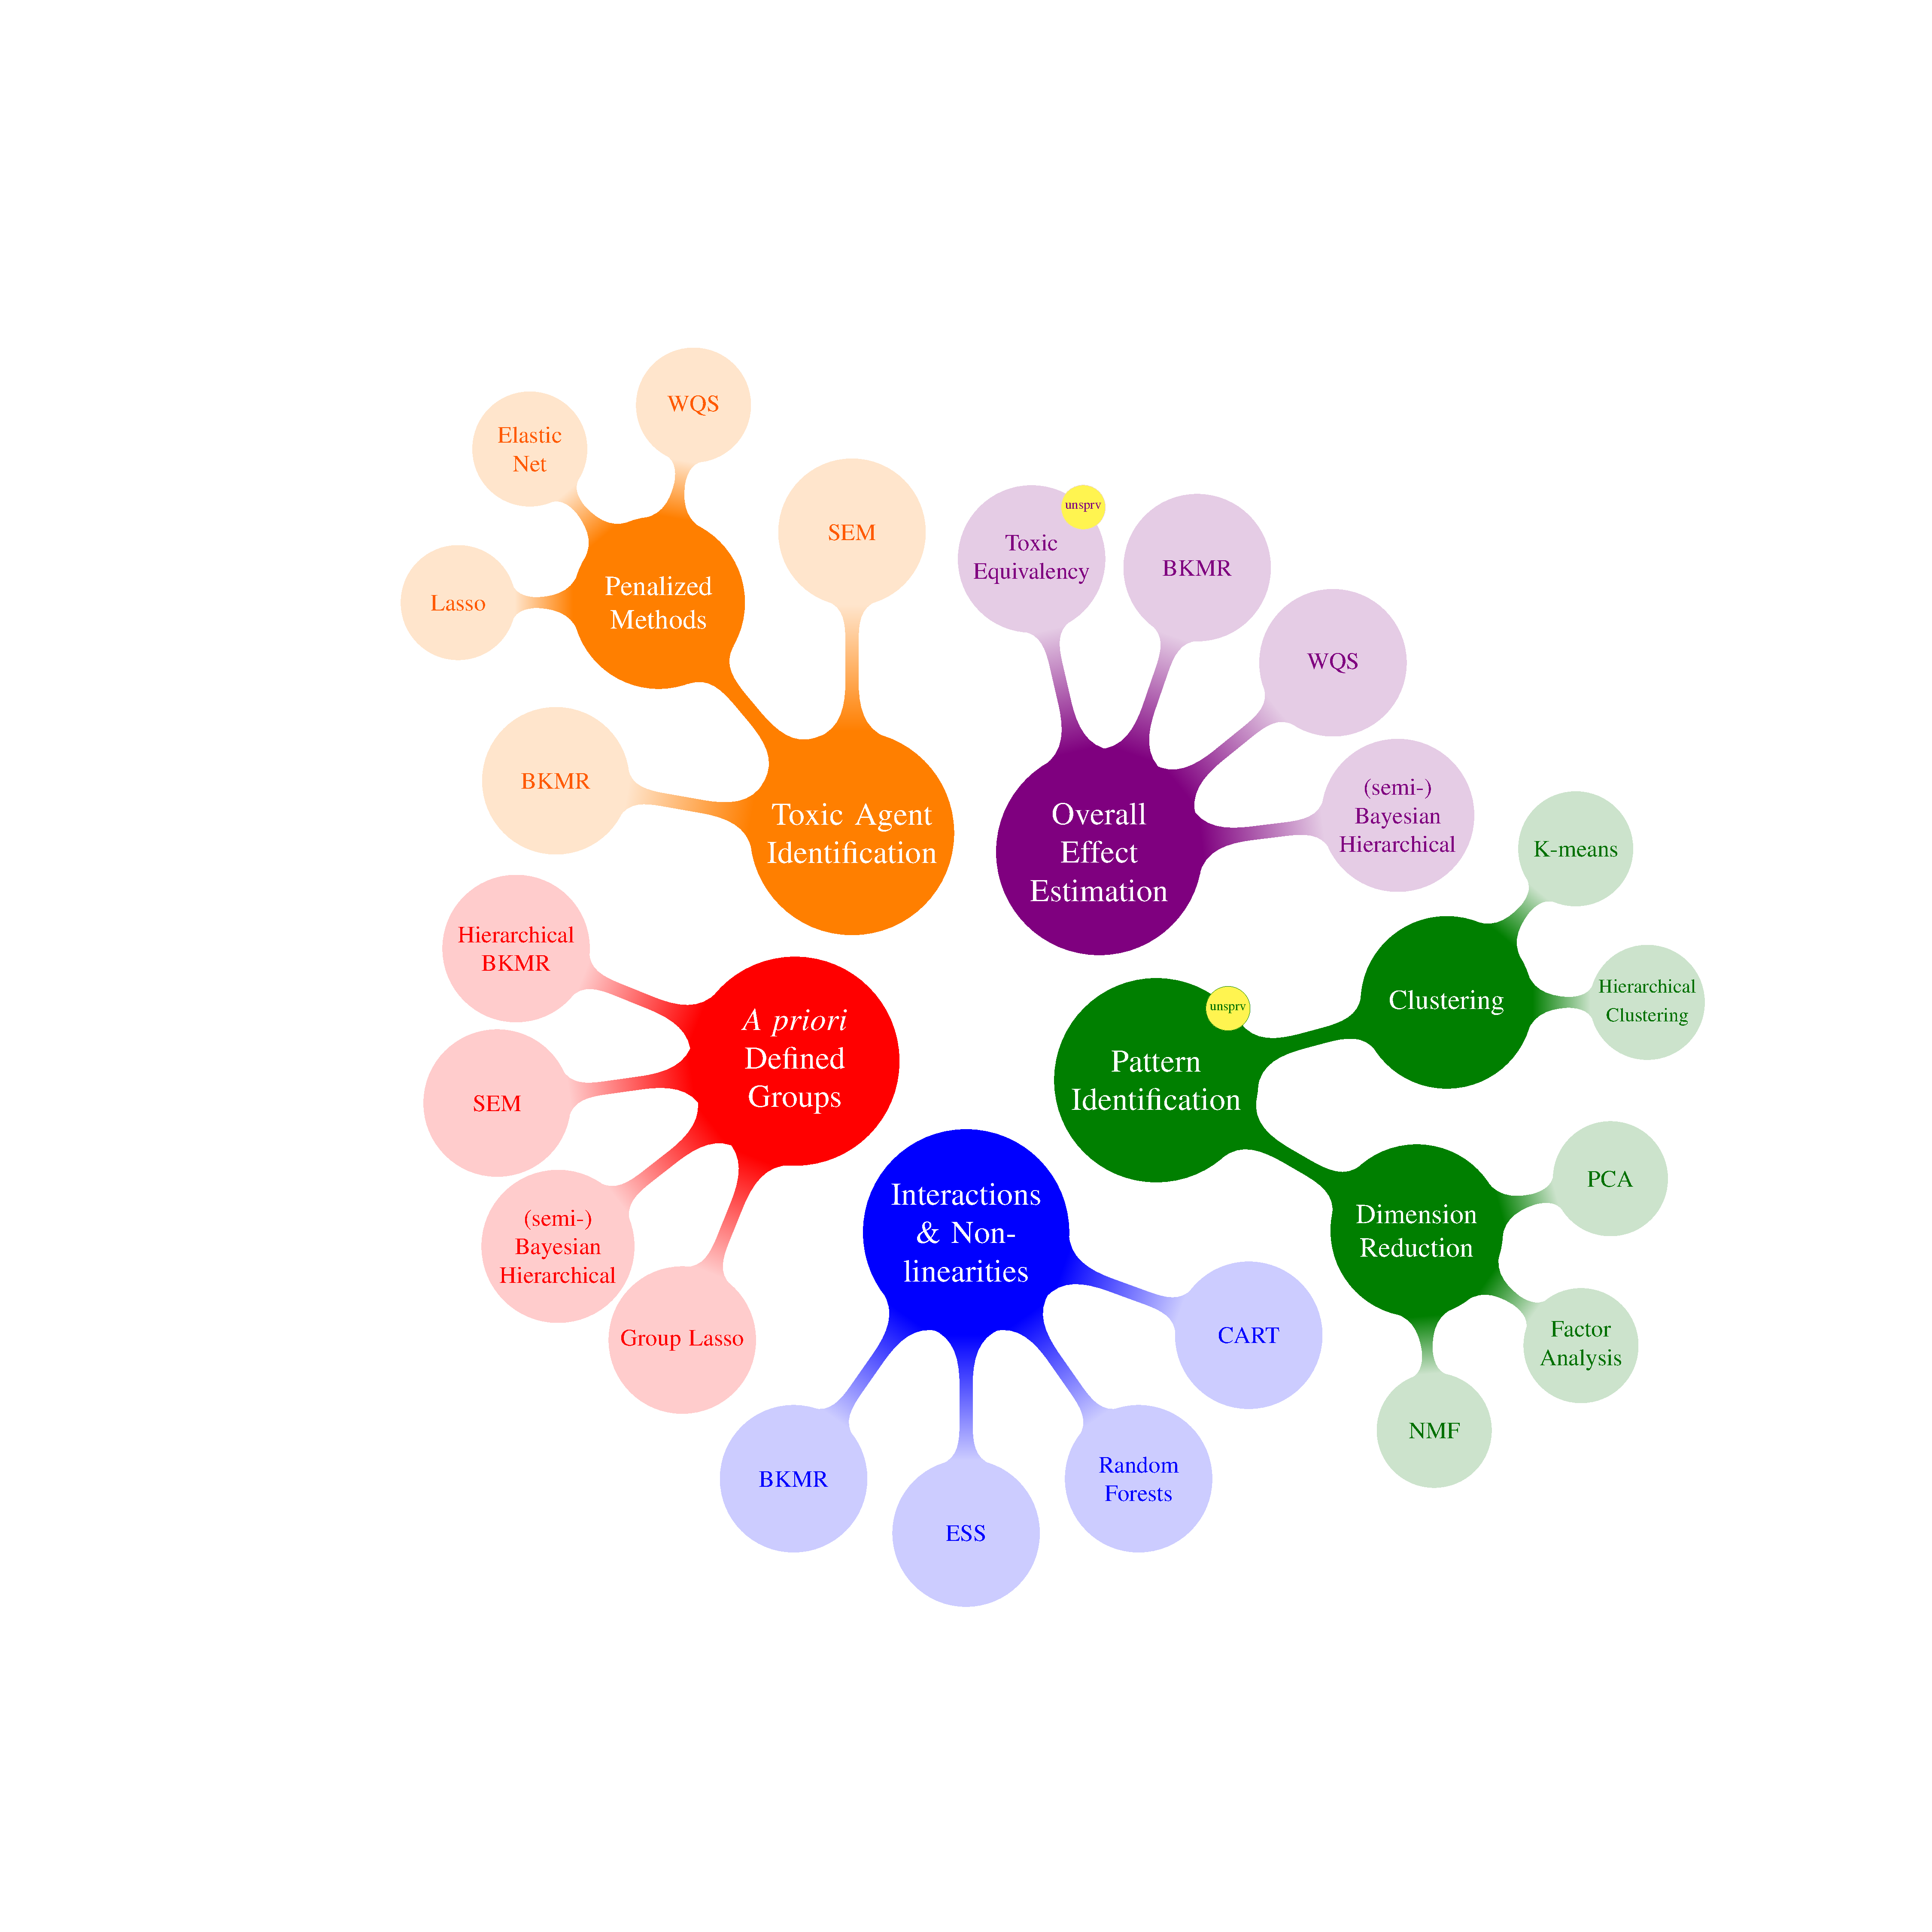
\includegraphics[height=6cm]{figures/overview.pdf}}}
\only<2>{{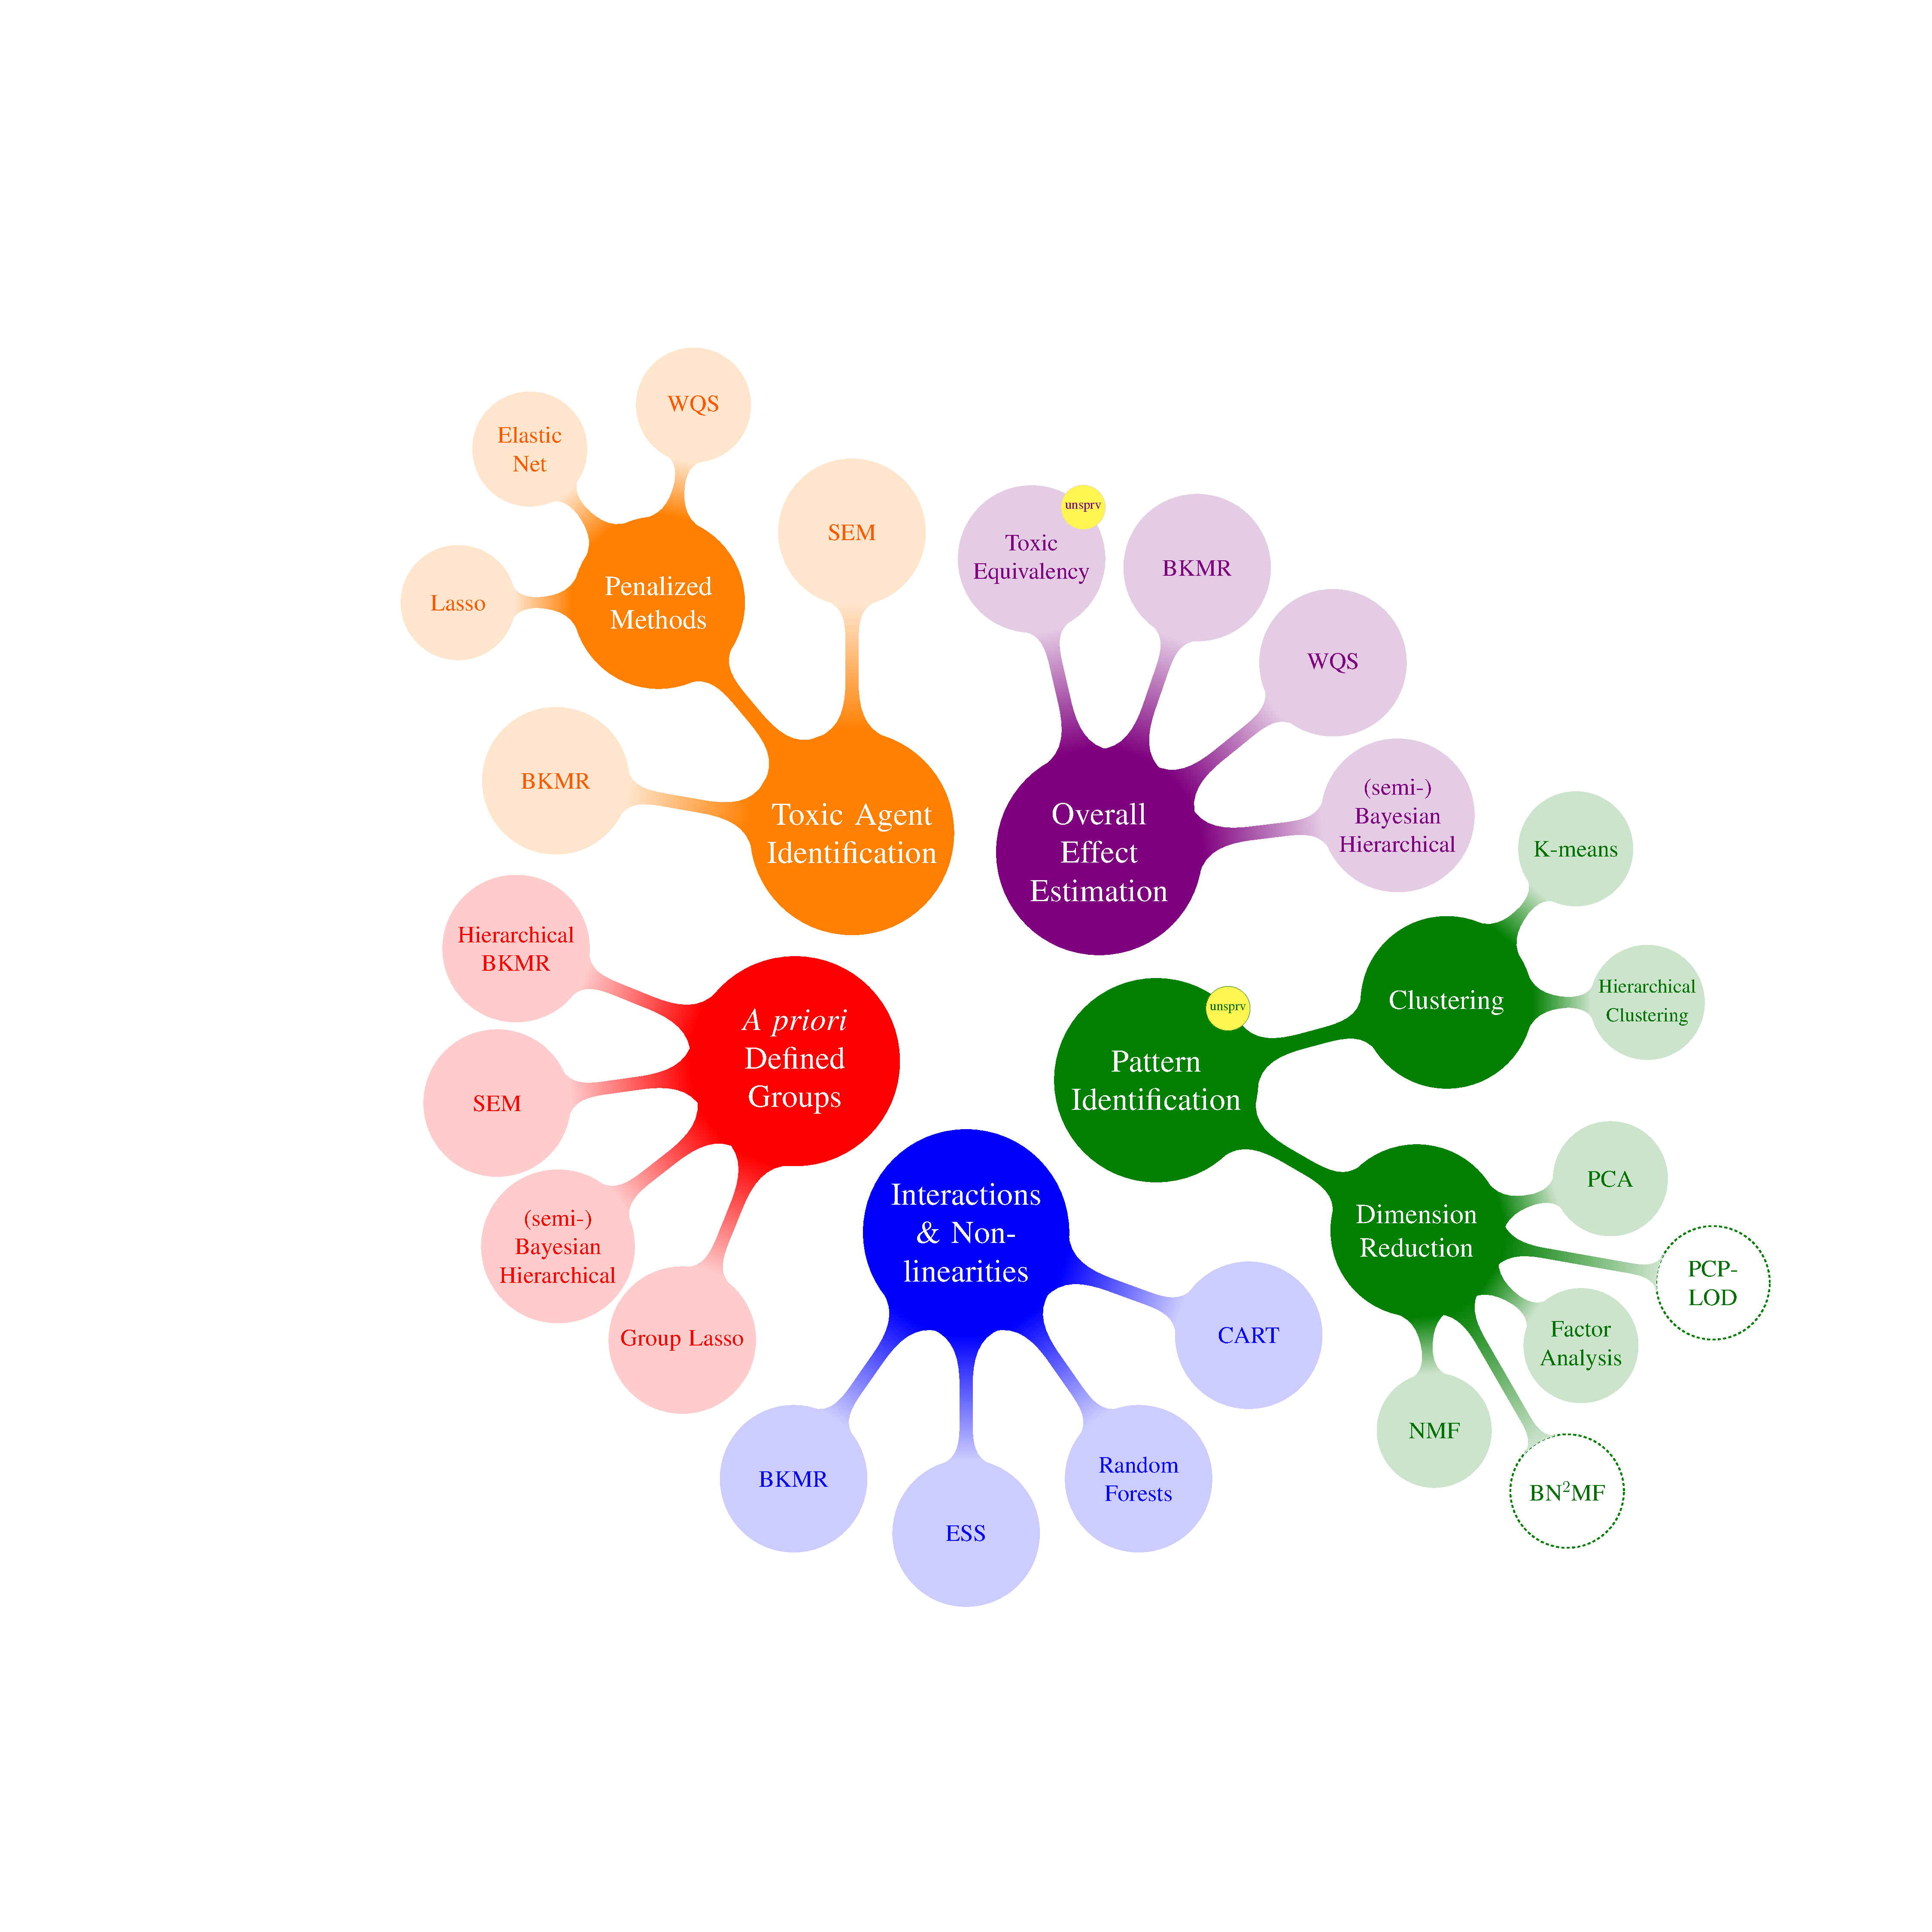
\includegraphics[height=6cm]{figures/Overview_add.pdf}}}
\end{changemargin}
{\tiny{\color{hgray}{$\ \hspace{9em} ^{\star}$Not an exhaustive list of methods!}}}
\end{columns}
}

